\chapter{Intersection Algorithms\label{intersect}}

In this chapter we are going to see a collection of algorithms to compute the intersection of two \textbf{sorted} lists, taken from the chapter six of "Pearl of Algorithm Engineering" by Paolo Ferragina, published by Cambridge University Press \citep{Ferragina_2023}. \\
We will first look at two of the most commonly used search algorithms, since we cannot intersect without searching. 

\section{Search Algorithms}

\subsection{Binary Search \label{sec:binsearch}}

\begin{figure}[H] 
    \begin{center}
        \includegraphics[width=.8\textwidth]{imgs/Binary_Search_Depiction.png}
        \caption{Binary search algorithm, source: \href{https://en.wikipedia.org/wiki/Binary_search}{Wikipedia}\label{fig:binsearch}}
    \end{center}
\end{figure}

Binary search, also known as logarithmic search or binary chop, is a search algorithm that locates the position of a target value within a sorted array: it compares the target to the middle element of the array and, if they are not equal, it eliminates half of the search space by discarding either the left or right half, depending on whether the target value is less than or greater than the middle element. This process is repeated by iteratively searching into the remaining sub-array until the target value is found or the search space is empty. The pseudocode for the algorithm can be seen at \textit{Algorithm} \brref{alg:binsearch}.\\
Binary search runs in logarithmic time in the worst case, doing $O(\log n)$ comparisons, where $n$ is the number of elements in the array, making it much faster than linear search with large arrays thanks to its scaling.

\begin{algorithm}
    \captionsetup{labelsep=newline}
    \caption{Pseudocode for binary search algorithm \label{alg:binsearch}}
    \begin{algorithmic}[1]
        \State Looking for element $key$
        \State Let $L=0$ \Comment{First half}
        \State Let $R=n-1$ \Comment{Second half}
        \While{$L\leq R$}
            \State $m=\lfloor (L+R)/2 \rfloor$
            \If{$A[M] < key$}
                \State let $L=m+1$
            \ElsIf{$A[M] > key$}
                \State $R = m - 1$
            \Else
                \State \Return $m$ \Comment{Found}
            \EndIf
        \EndWhile
        \State \Return False \Comment{Not found}
    \end{algorithmic}
\end{algorithm}

\subsection{Exponential Search \label{sec:expsearch}}

\begin{figure}[H] 
    \begin{center}
        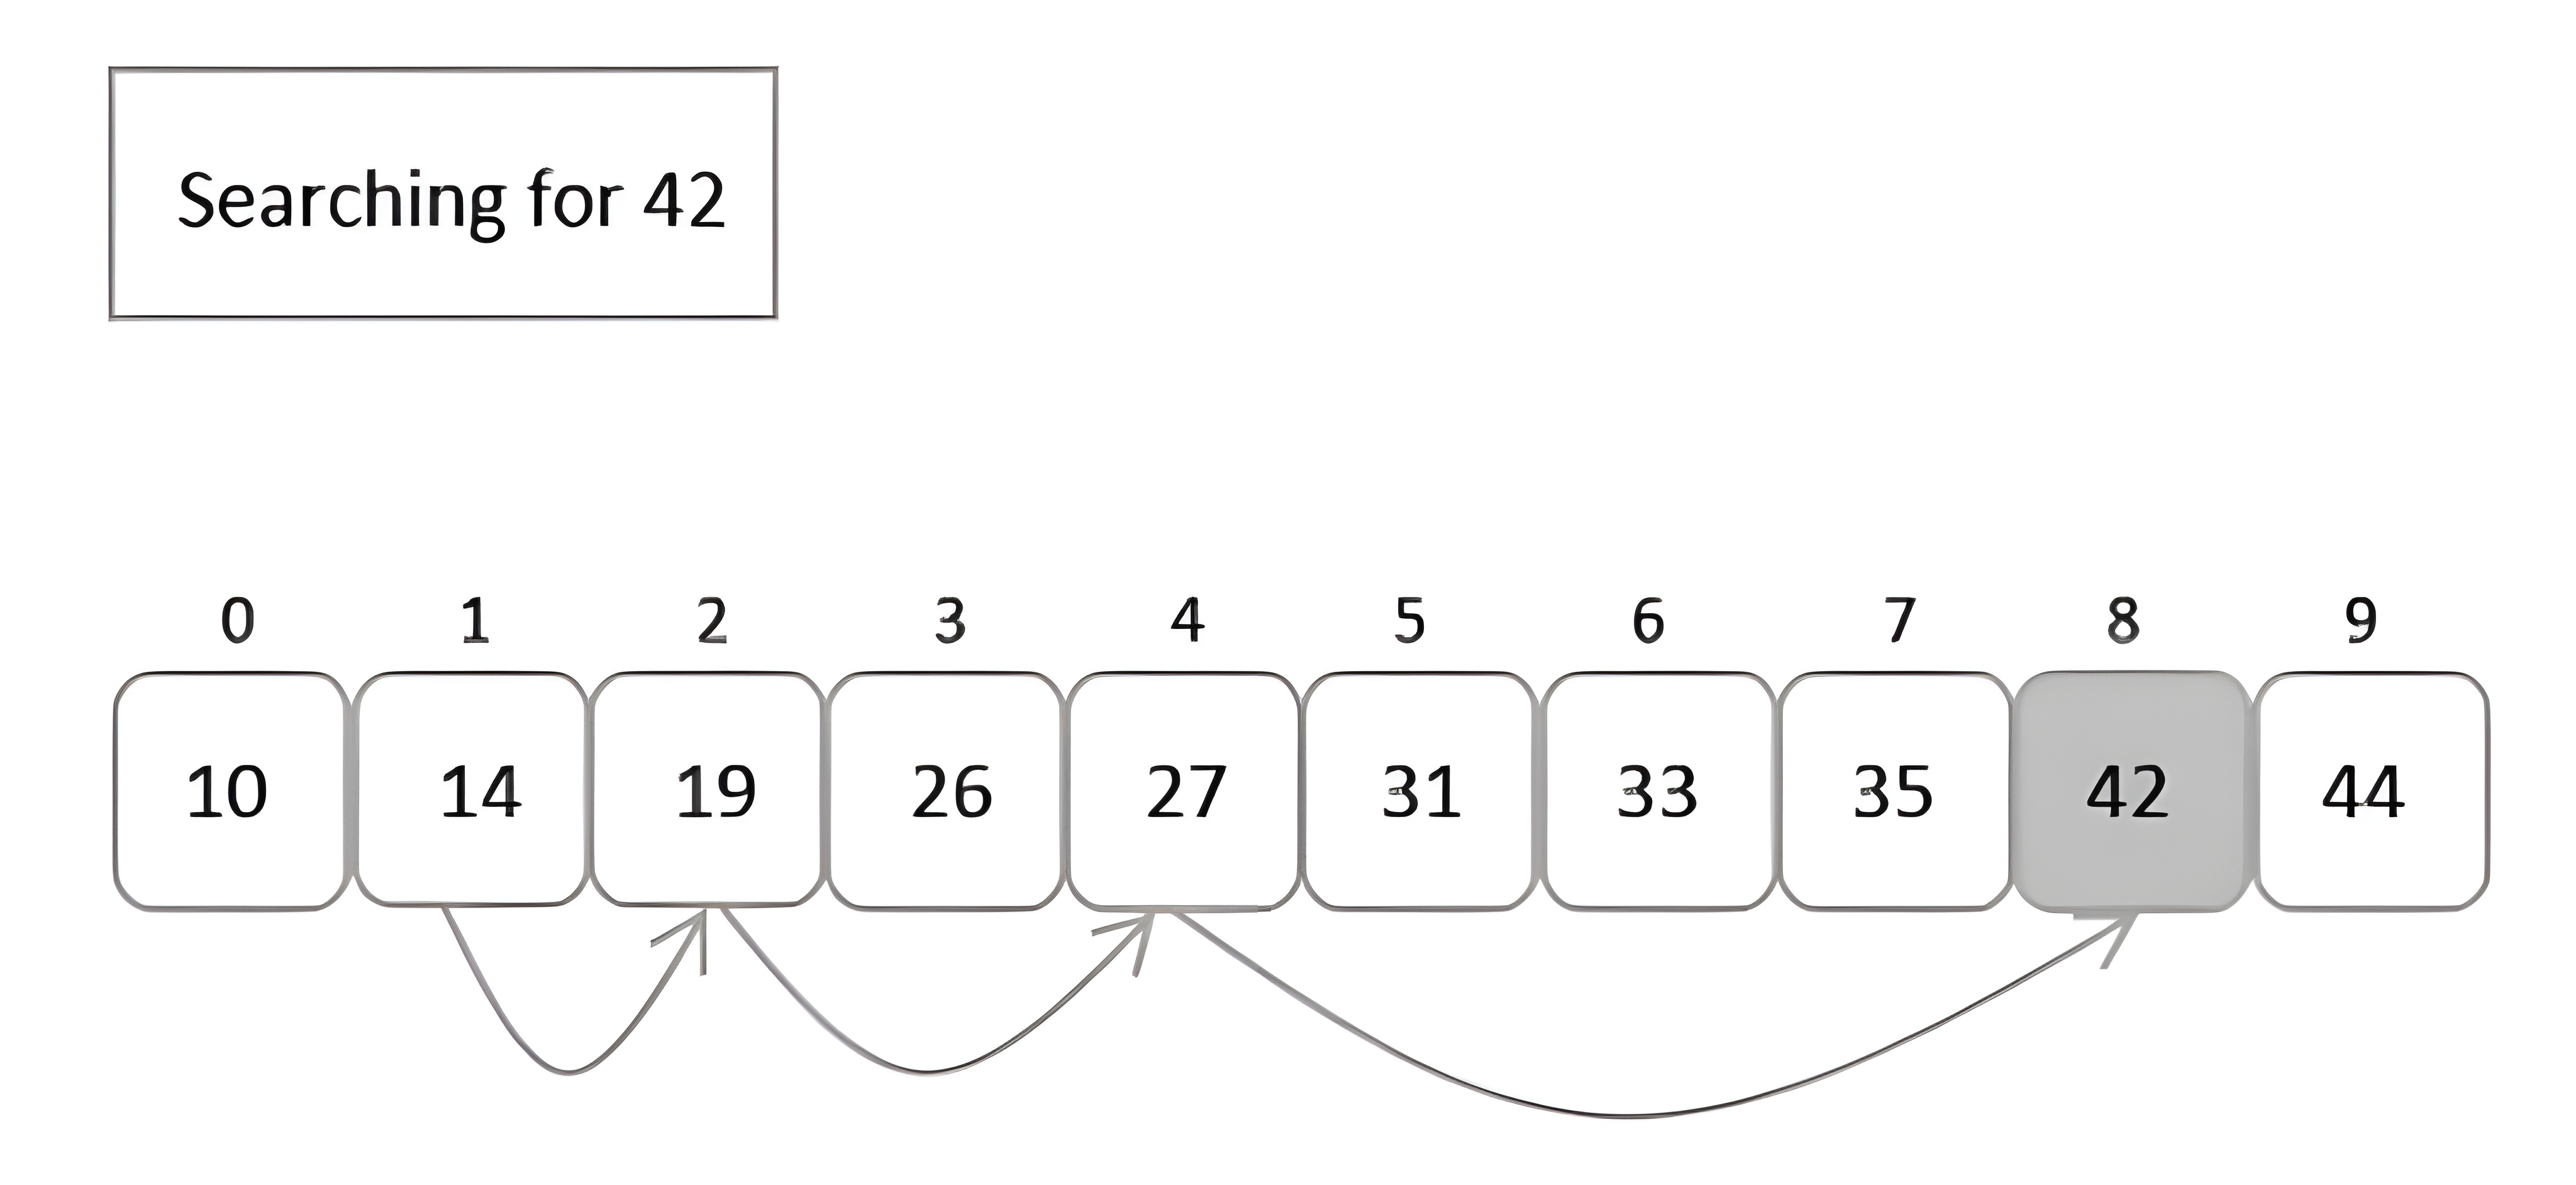
\includegraphics[width=.8\textwidth]{imgs/exponential_search.png}
        \caption{Exponential search algorithm, source: \href{https://www.tutorialspoint.com/data_structures_algorithms/exponential_search.htm}{Tutorialspoint}\label{fig:expsearch}}
    \end{center}
\end{figure}

Exponential search, also called doubling or galloping search, is an algorithm for searching sorted, unbounded lists: there are numerous implementations, most common being determining a sub-array into which the \verb|key| may resides in and performing a binary search \brref{sec:binsearch} within its range.\\
To be more precise: we examine the list in exponentially increasing steps, with a factor of $2^k$ such that we first look into \verb+list[0]+, then \verb+list[1]+, then \verb+list[2]+, \verb+list[4]+, \verb+list[8]+, following with \textit{16}, \textit{32}, \textit{64}, \textit{128} and so on until we find a value that is greater than the \verb|key|. Once we find it, we perform a binary search between the previous step and the current (or the end of the array): $2^{k-1} \leq key \leq min(2^{k},n)$.

The algorithm can be more efficient than binary search, as it runs in $O(\log i)$ time, where $i$ is the index of the element being searched for, which could be half if not less than $n$.\\
The pseudocode can be seen at \textit{Algorithm} \brref{alg:expsearch}.

\begin{algorithm}
    \captionsetup{labelsep=newline}
    \caption{Pseudocode for exponential search algorithm \label{alg:expsearch}}
    \begin{algorithmic}[1]
        \State Looking for element $key$
        \State Let $i=0$ 
        \State Let $k=0$
        \While{($key>list[i+2^k]$ and $i<n$)} 
            \State $i=i+2^k$ \Comment Gallop to next step
            \State $k=k+1$ \Comment Increment exponent
        \EndWhile
        \If{$i<n$}
            \State binary\_search($list$, $key$, $i$, $min(i+2^k,n)$) 
        \Else
            \State \Return false \Comment{Not found}
        \EndIf
    \end{algorithmic}
\end{algorithm}

\section{Intersection Algorithms}

\subsection{Brute Force \label{sec:bruteforce}}

The first idea that would come to mind when thinking about intersecting two lists is to simply iterate through both of them and check for matching elements: this is the \textit{brute force} approach, which is simple but inefficient. \\
With a time complexity of $O(m \cdot n)$, assuming lists sizes $n$ and $m$ to be around $10^6$, and assuming a modern computer able to do $10^9$ operations per second, this algorithm would need ten minutes to compute a 2-words query, which is less than ideal.\\
The (very short) pseudocode can be seen at \textit{Algorithm} \brref{alg:bruteforce}.

\begin{algorithm}
    \captionsetup{labelsep=newline}
    \caption{Pseudocode for brute force algorithm \label{alg:bruteforce}}
    \begin{algorithmic}[1]
        \ForAll{$i=0$ to $n-1$}
            \ForAll{$j=0$ to $m-1$}
                \If{$A[i] == B[j]$}
                    \State add $A[i]$ to result
                \EndIf
            \EndFor
        \EndFor
    \end{algorithmic}
\end{algorithm}

\subsection{Bunny Race \label{sec:bunnyrace}}

\begin{figure}[H] 
    \begin{center}
        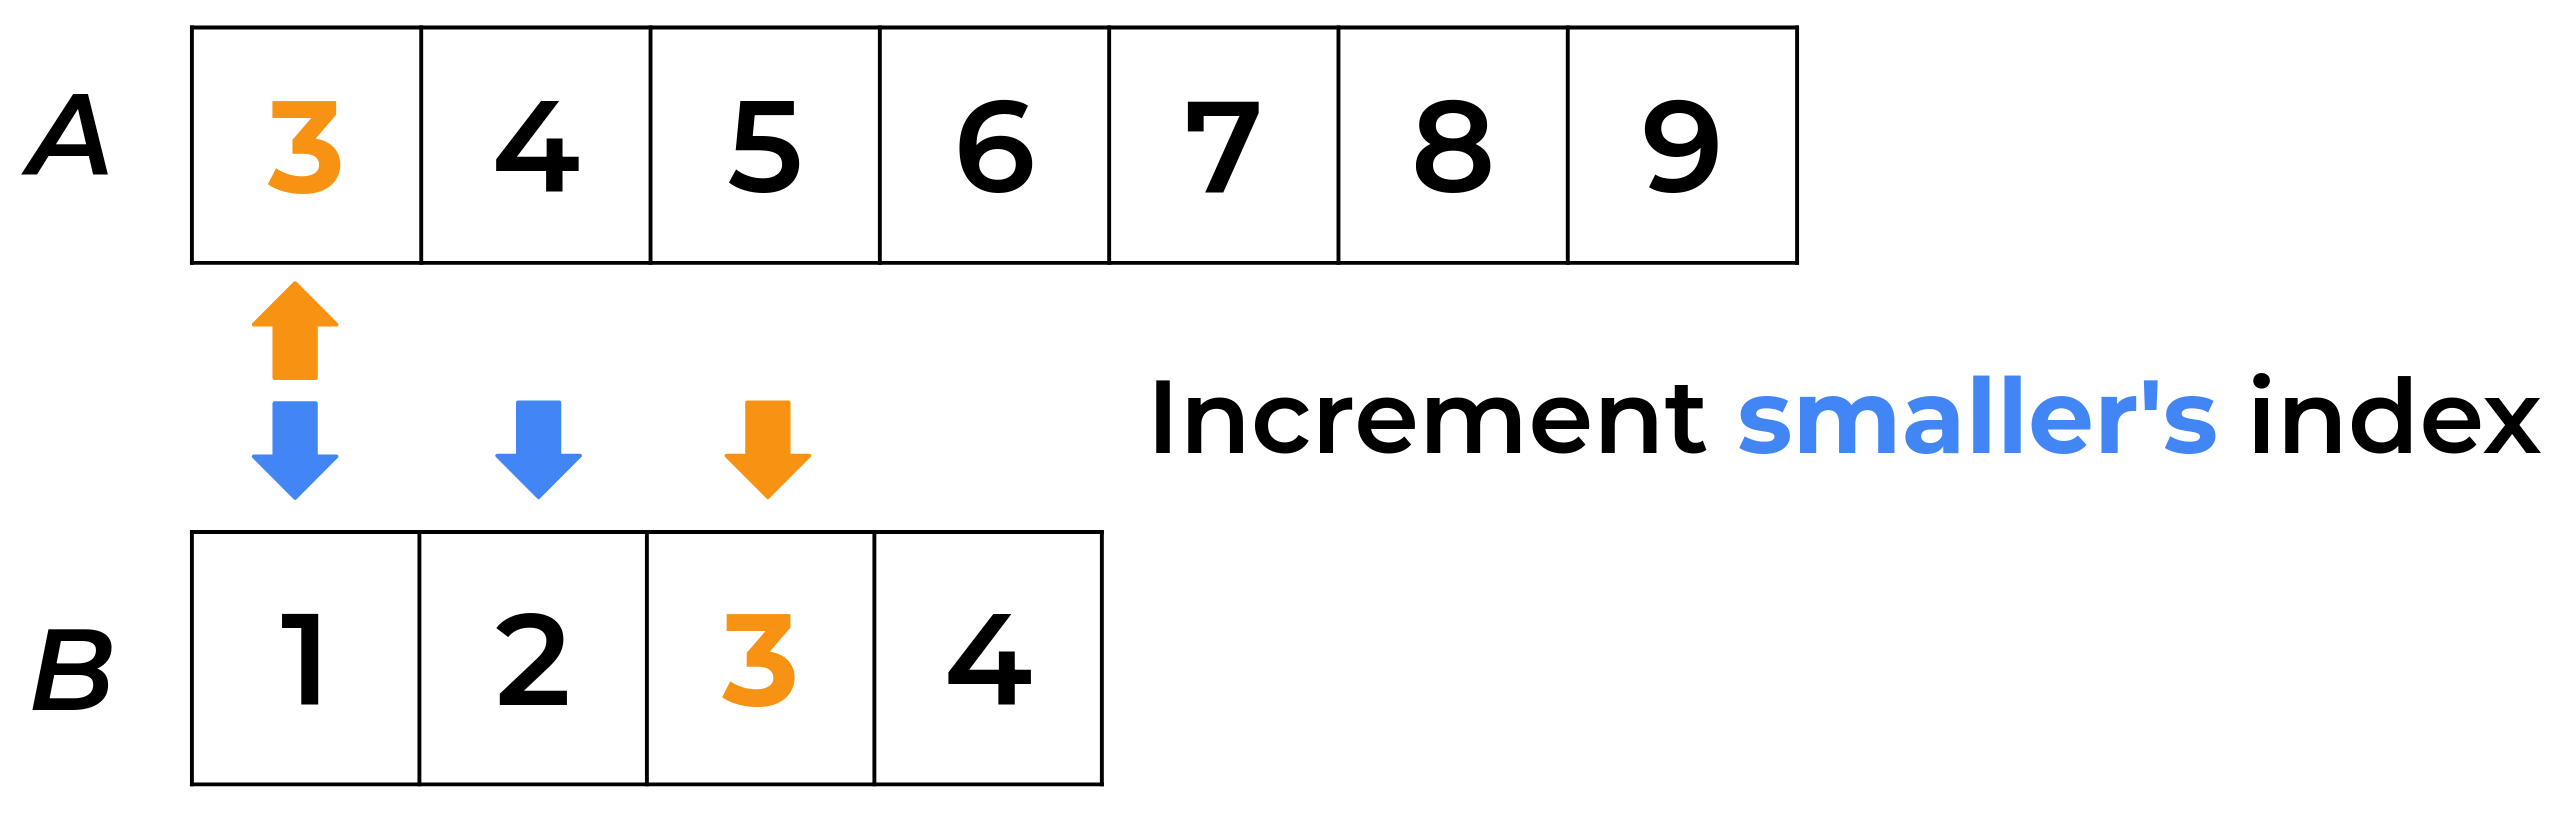
\includegraphics[width=.8\textwidth]{imgs/bunny_search.png}
        \caption{Bunny race algorithm \label{fig:bunnyrace}}
    \end{center}
\end{figure}

This approach, often called merge-based, is simple, elegant and fast: the main idea is to have two indices pointing at the two list running after each other by comparing elements each time and incrementing the index pointing at the smallest one (or incrementing both if they are equal).\\ 
To clarify: lets say we have two lists, $A$ and $B$, of size $n$ and $m$ respectively. We start with two pointers, $i$ and $j$, both set to zero. \\
We compare the elements at these indices, $A[i]$ and $B[j]$: if they are equal, we add the element to the result and increment both pointers. \\
If $A[i] < B[j]$, we increment $i$, while if $A[i] > B[j]$, we increment $j$. \\
This process continues until one of the pointers reaches the end of its respective list.\\
The correctness can be proven inductively, exploiting the following observation: if $A[i] < B[j]$ then $A[i]$ is smaller than all elements following $B[j]$ in $B$ since its ordered, so $A[i] \notin B$. The other case is symmetric. \\
In regards to time complexity, we just need to note that at each step the algorithm executes one comparison and advances at least one iterator, thus, given that $n=|A|$ and $m=|B|$, the algorithm runs in no more than $O(n+m)$ time.\\
This time complexity is significantly better than the \textit{brute force} \brref{alg:bruteforce} approach, since it can compute a 2-word query in $10^{-3}$ seconds. \\
The pseudocode can be seen at \textit{Algorithm} \brref{alg:bunnyrace}.

In the case that $n=\Theta (m)$ this algorithm is optimal, because we need to process the smallest set, thus $\Omega(min(n,m))$ is an obvious lower bound. Moreover, this procedure is also optimal in the disk model since it takes $O \left(\frac{n}{B}\right)$ I/Os. \\
In the case that $n \ll m$ the classic \textit{binary search} can be helpful since we can design an algorithm that search in $A$ for each elements of $B$ in $O(m \log n)$ time, which is better than $O(n+m)$ when $m=o\left(\frac{n}{\log n}\right)$.

\begin{algorithm}
    \captionsetup{labelsep=newline}
    \caption{Pseudocode for bunny race algorithm \label{alg:bunnyrace}}
    \begin{algorithmic}[1]
        \State Let $i=0$ 
        \State Let $j=0$ 
        \While{$i<n$ and $j<m$}
            \If{$A[i] < B[j]$}
                \State $i=i+1$ \Comment Increment first
            \ElsIf{$A[i] > B[j]$}
                \State $j=j+1$ \Comment Increment second
            \Else
                \State Add $A[i]$ to result \Comment Found
                \State $i=i+1$  \Comment Increment both
                \State $j=j+1$
            \EndIf
        \EndWhile
    \end{algorithmic}
\end{algorithm}

\subsection{Divide and Search \label{sec:divandsearch}}

\begin{figure}[H] 
    \begin{center}
        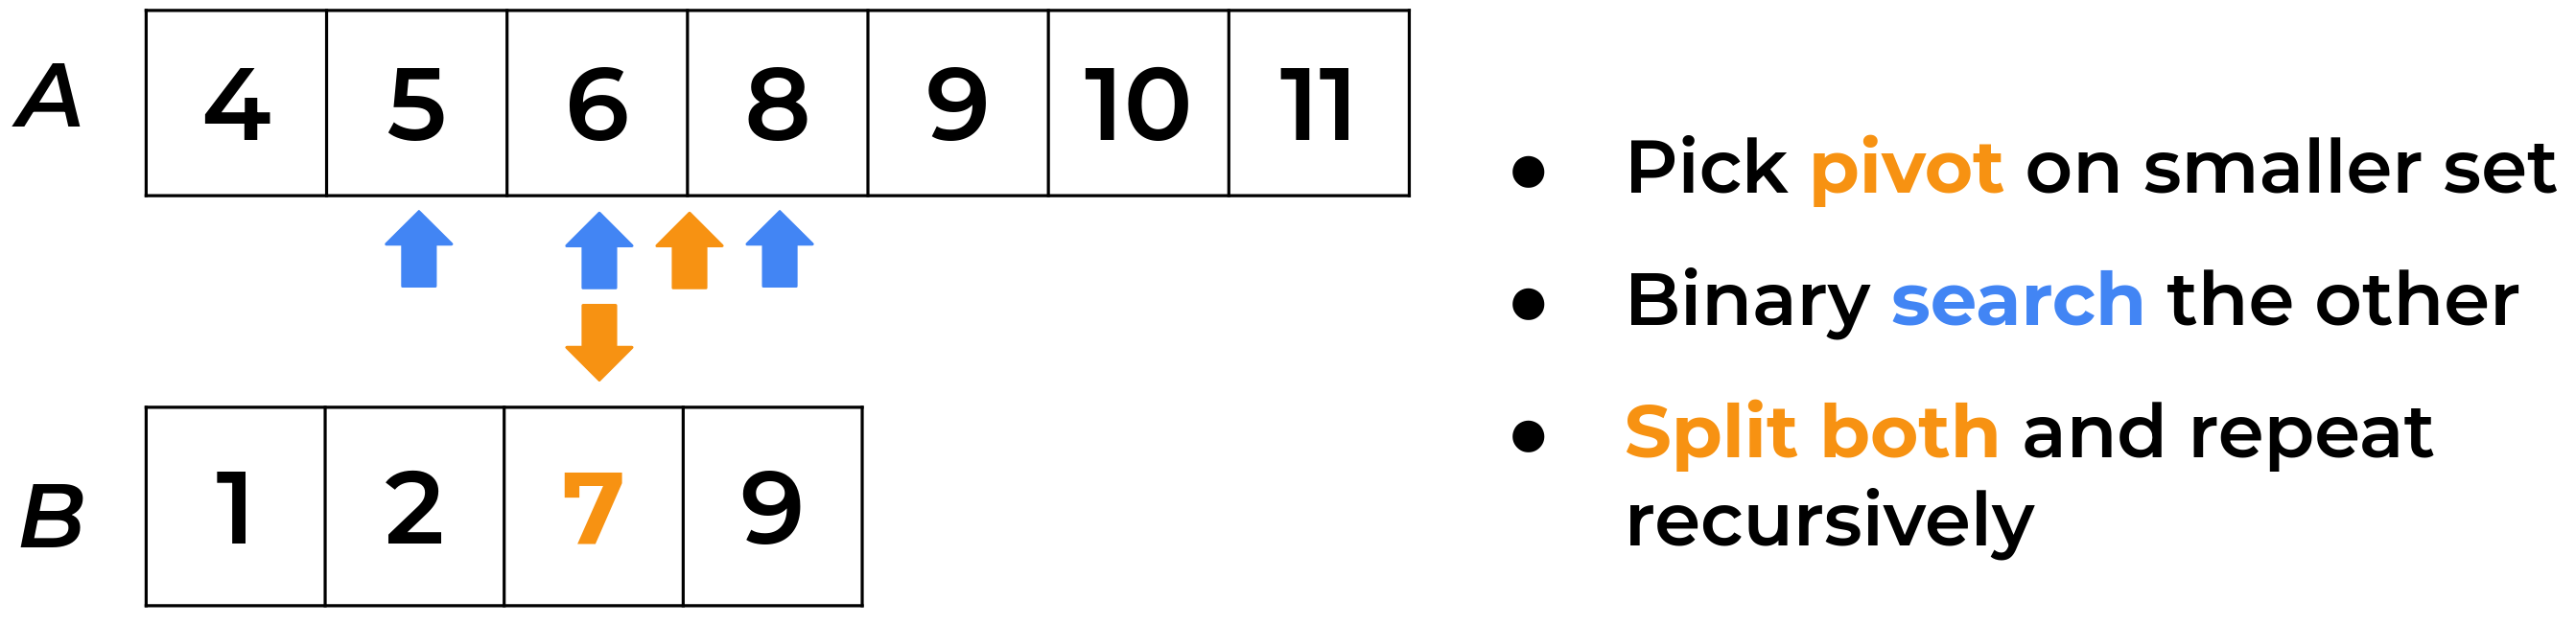
\includegraphics[width=.8\textwidth]{imgs/divide_and_search.png}
        \caption{Divide and search algorithm \label{fig:divandsearch}}
    \end{center}
\end{figure}

Also called \textit{mutual partitioning}, this approach adopts a classic algorithmic paradigm, namely \textit{divide and conquer}, famously used to design the \textit{quick sort} algorithm (which can be visualized \href{https://en.wikipedia.org/wiki/Quicksort}{here}).\\
Let us assume $m=|B| \leq n=|A|$. We select the median element of $B$, $b_{m/2}$, as a \textit{pivot} and search for it in the longer sequence $A$ using the \textit{binary search} \brref{sec:binsearch} algorithm.
Two cases may occur: 

\begin{itemize}
    \item[i.] \textit{pivot} is one of the elements fo the intersection;
    \item[ii.] $b_{m/2} \notin A$, e.g, $A[j]<b_{m/2}<A[j+1]$.
\end{itemize}

In both cases the algorithm proceeds \textit{recursively} by calling itself on the two sub-lists in which each list ($A$ and $B$) has been split according to the \textit{pivot} element, thus computing the following intersections:

\begin{itemize}
    \item $A\big[1, j\big] \cap B\big[1, \frac{m}{2}-1\big]$
    \item $A\big[ j+1, n\big] \cap B\big[\frac{m}{2}+1, m\big]$.
\end{itemize}

In simpler terms: we pick the middle element of the smaller list, search for it in the bigger list, split both lists and repeat the process recursively on the remaining sub-lists, then again, then again, then again, until we reach the base case where each list is of size one.\\
The pseudocode of the algorithm can be seen at \textit{Algorithm} \brref{alg:divandsearch}.

Correctness follows, while for evaluating time complexity we need to identify the worst case. \\
Let us start with the case where \textit{pivot} falls outside \textit{A}, meaning that one of the two parts is empty and thus the corresponding half of \textit{B} can be ignored. So, one \textit{binary search} \brref{sec:binsearch} over \textit{A}, costing $O(\log n)$ time, has discarded half of \textit{B}.\\
If this keeps occurring in all recursive calls, the total number of them will be $O(\log m)$, which leads us to a time complexity of $O(\log m \log n)$.\\
On the other hand, if we have both balanced partitions so that $b_{m/2}$ not only falls inside \textit{A} but coincides with the median element $a_{n/2}$, the time complexity can be expressed via the recurrence relation $T(n, m) = O(\log n) + 2T \left(\frac{n}{2}, \frac{m}{2}\right)$, with the base case $T(n,m)=O(1)$ whenever $n,m \leq 1$.\\
This recurrence has the solution $T(n,m)=O \big(m \big(1+\log \frac{n}{m}\big)\big)$ for each $m \leq n$, which is an optimal time complexity in the comparison model.

That being said, despite its optimal time complexity, the mutual-partitioning paradigm is heavily based on recursive calls and binary searching, and both paradigms offer poor performance in a disk-based setting when sequences are long hence requiring a large number of both dynamic memory allocations (recursive calls) and random memory access (\textit{binary search} steps).

\begin{algorithm}
    \captionsetup{labelsep=newline}
    \caption{Pseudocode for divide and search algorithm \label{alg:divandsearch}}
    \begin{algorithmic}[1]
        \State Let $m=|B| \leq n=|A|$
        \State Pick \textit{pivot} $p=b_{\lfloor m/2 \rfloor}$
        \State \textit{Binary search} for \textit{p} in \textit{A} \Comment Say $a_j \leq p < a_{j+1}$
        \State \textit{Divide and search} on $A\big[1, j\big] \cap B\big[1, \frac{m}{2}-1\big]$
        \If{$p=a_j$}
            \State Add \textit{p} to result
        \EndIf
        \State \textit{Divide and search} on $A\big[ j+1, n\big] \cap B\big[\frac{m}{2}+1, m\big]$
    \end{algorithmic}
\end{algorithm}

\subsection{Doubling Search \label{galloping}}

\begin{figure}[H] 
    \begin{center}
        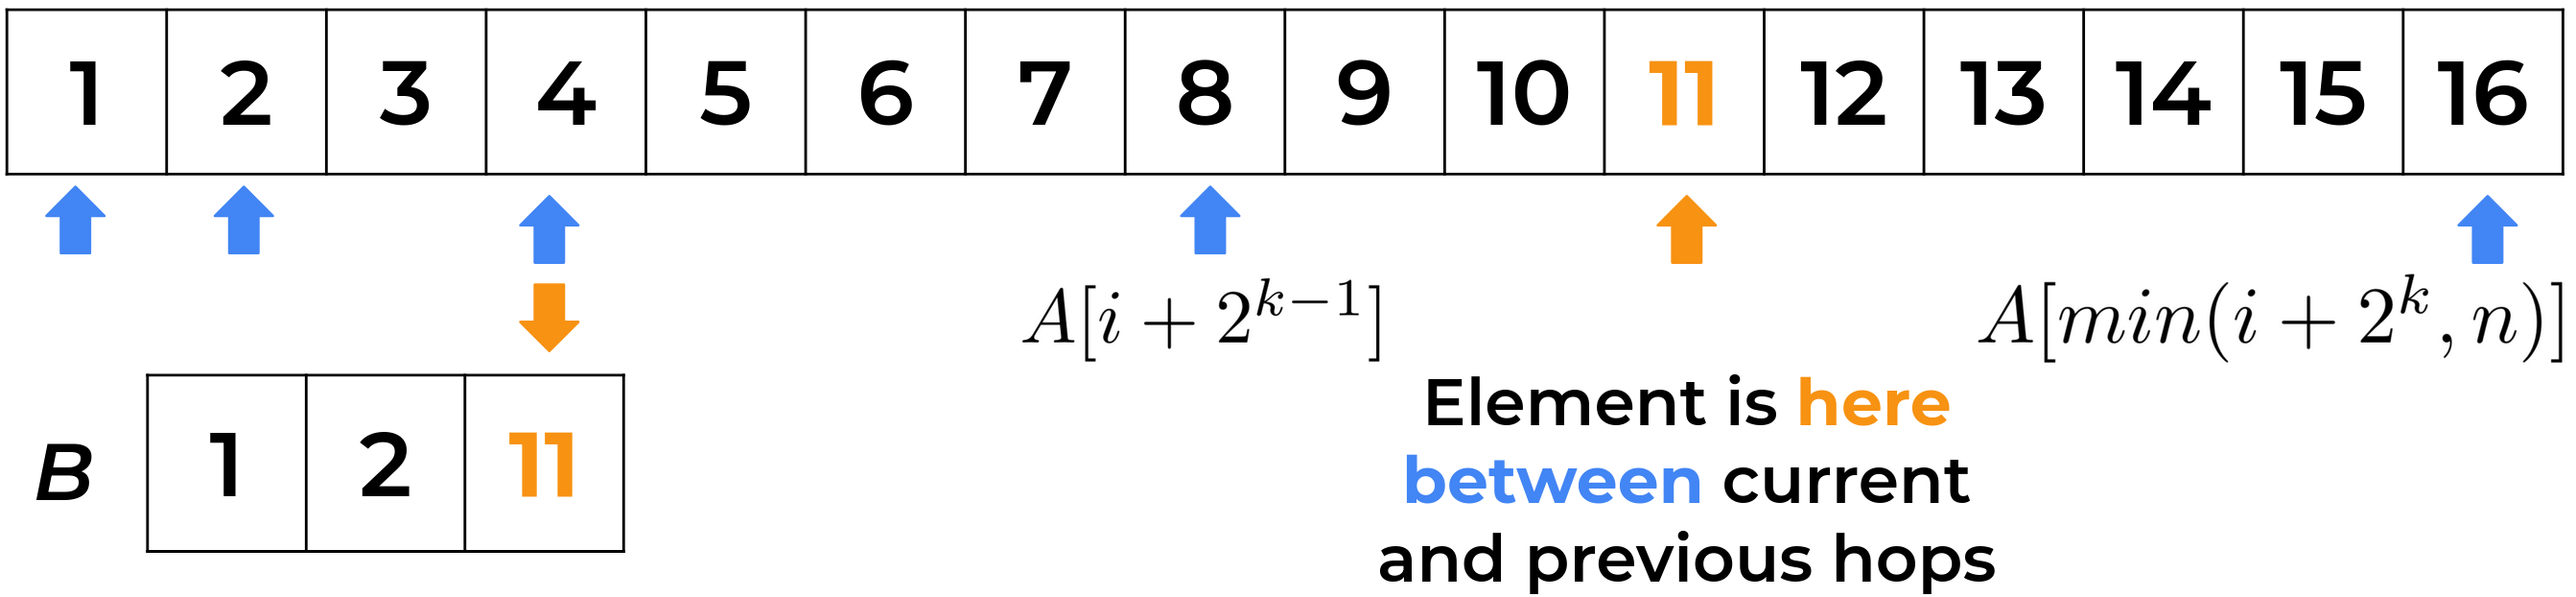
\includegraphics[width=.8\textwidth]{imgs/galloping.png}
        \caption{Doubling search algorithm \label{fig:galloping}}
    \end{center}
\end{figure}

Also called \textit{exponential search} or \textit{galloping search}, this paradigm is more or less what we presented in the search algorithm \textit{exponential search} \brref{sec:expsearch}: assuming $m=|B| \leq n=|A|$, we search of each element $b_j$ of \textit{B} into \textit{A} by jumping trough it with exponentially bigger steps that increase by a factor of $2^k$, meaning that we compare $b_j$ with $A[0]$, $A[1]$, $A[2]$, $A[4]$, $A[8]$, $A[16]$, $A[32]$, and so on, until we find that either $b_j<A\left[i+2^k\right]$ for some \textit{k}, or we have jumped out of the array since $i+2^k>n$.\\
Then we perform a \textit{binary search} \brref{sec:binsearch} for $b_j$ between $A\left[i+2^{k-1}\right]$ and $A\left[min\left(i+2^k, n\right)\right]$. $A\left[0, i+2^{k-1}\right]$ will be discarded from the subsequent searches.\\
The pseudocode of the algorithm can be seen at \textit{Algorithm} \brref{alg:galloping}, which is a bit different from the one we saw in \textit{exponential search} section \brref{sec:expsearch}, so it can be seen as an extra resource. Both works very similarly.

Correctness is again immediate, while deriving time complexity will require some reasoning: we denote with $\Delta_i$ the size of the sub-array of \textit{A} where $b_j$ could be found.
We then say that:
\begin{itemize} 
    \item $b_j \geq i+2^{k-1}$ i.e. previous step
    \item $b_j<min\left(i+2^k,n\right)$ i.e. current step or end of \textit{A}
\end{itemize}

We can therefore write $2^{k-1} \leq i-(i-1)$ where $i$ and $(i-1)$ are current and previous step respectively, and combining this inequality with $\Delta_i$ we get $\Delta_i \leq 2^{k-1} \leq i-(i-1)$. \\
At this point we can estimate the total length of search sub-arrays of \textit{A}: $\sum_{i=1}^{m} \Delta_i \leq \sum_{i=1}^{m} (i-(i-1)) \leq n$, because the latter is a telescopic sum in which consecutive terms cancel out.\\
For every \textit{i}, the algorithm executes $O\left(1+ \log \Delta_i\right)$ steps, thus summing for $i = 1,2,...,m$ (since $m=|B|$) we get a total time complexity of:\\
$\sum_{i=1}^m O\left(1+ \log \Delta_i\right)=O\left(\sum_{i=1}^{m}\left(1+log \Delta_i\right)\right)=O\left(m+m \log \sum_{i=1}^m \frac{\Delta_i}{m}\right)=O\left(m\left(1+ \log \frac{n}{m}\right)\right)$.\\
This is the same time complexity we got from the \textit{divide and search} \brref{alg:divandsearch} algorithm, except with a iterative paradigm, which thus does not require dynamic memory allocation. Moreover, it calls the \textit{binary search} \brref{sec:binsearch} on a sub-array of \textit{A} needing less disk accesses. Unfortunately, it falls short with very large lists, since galloping through them may require moving them in chunks back and forth from memory. It would thus be ideal to \textit{compress} in some way the vector \textit{A}.

\begin{algorithm}
    \captionsetup{labelsep=newline}
    \caption{Pseudocode for doubling search algorithm \label{alg:galloping}}
    \begin{algorithmic}[1]
        \State Let $m=|B| \leq n=|A|$
        \State Let $i=0$
        \ForAll{$j=0$ to $m-1$}
            \State Let $k=0$
            \While{$B\big[j\big] > A\big[i+2^k\big]$ and $i+2^k \leq n$}
                \State $k=k+1$ \Comment Increment exponent
            \EndWhile
            \State $i'$ = \textit{binary search} into $A\left[i+2^{k-1}+1, min\left(i+2^k\right),n\right]$
            \If{$a_{i'}=b_j$}
                \State Add $b_j$ to result
            \EndIf
            \State $i=i'$ \Comment Update $i$ to the last position
        \EndFor
    \end{algorithmic}
\end{algorithm}

\subsection{Two-Level Storage Approach}

\begin{figure}[H] 
    \begin{center}
        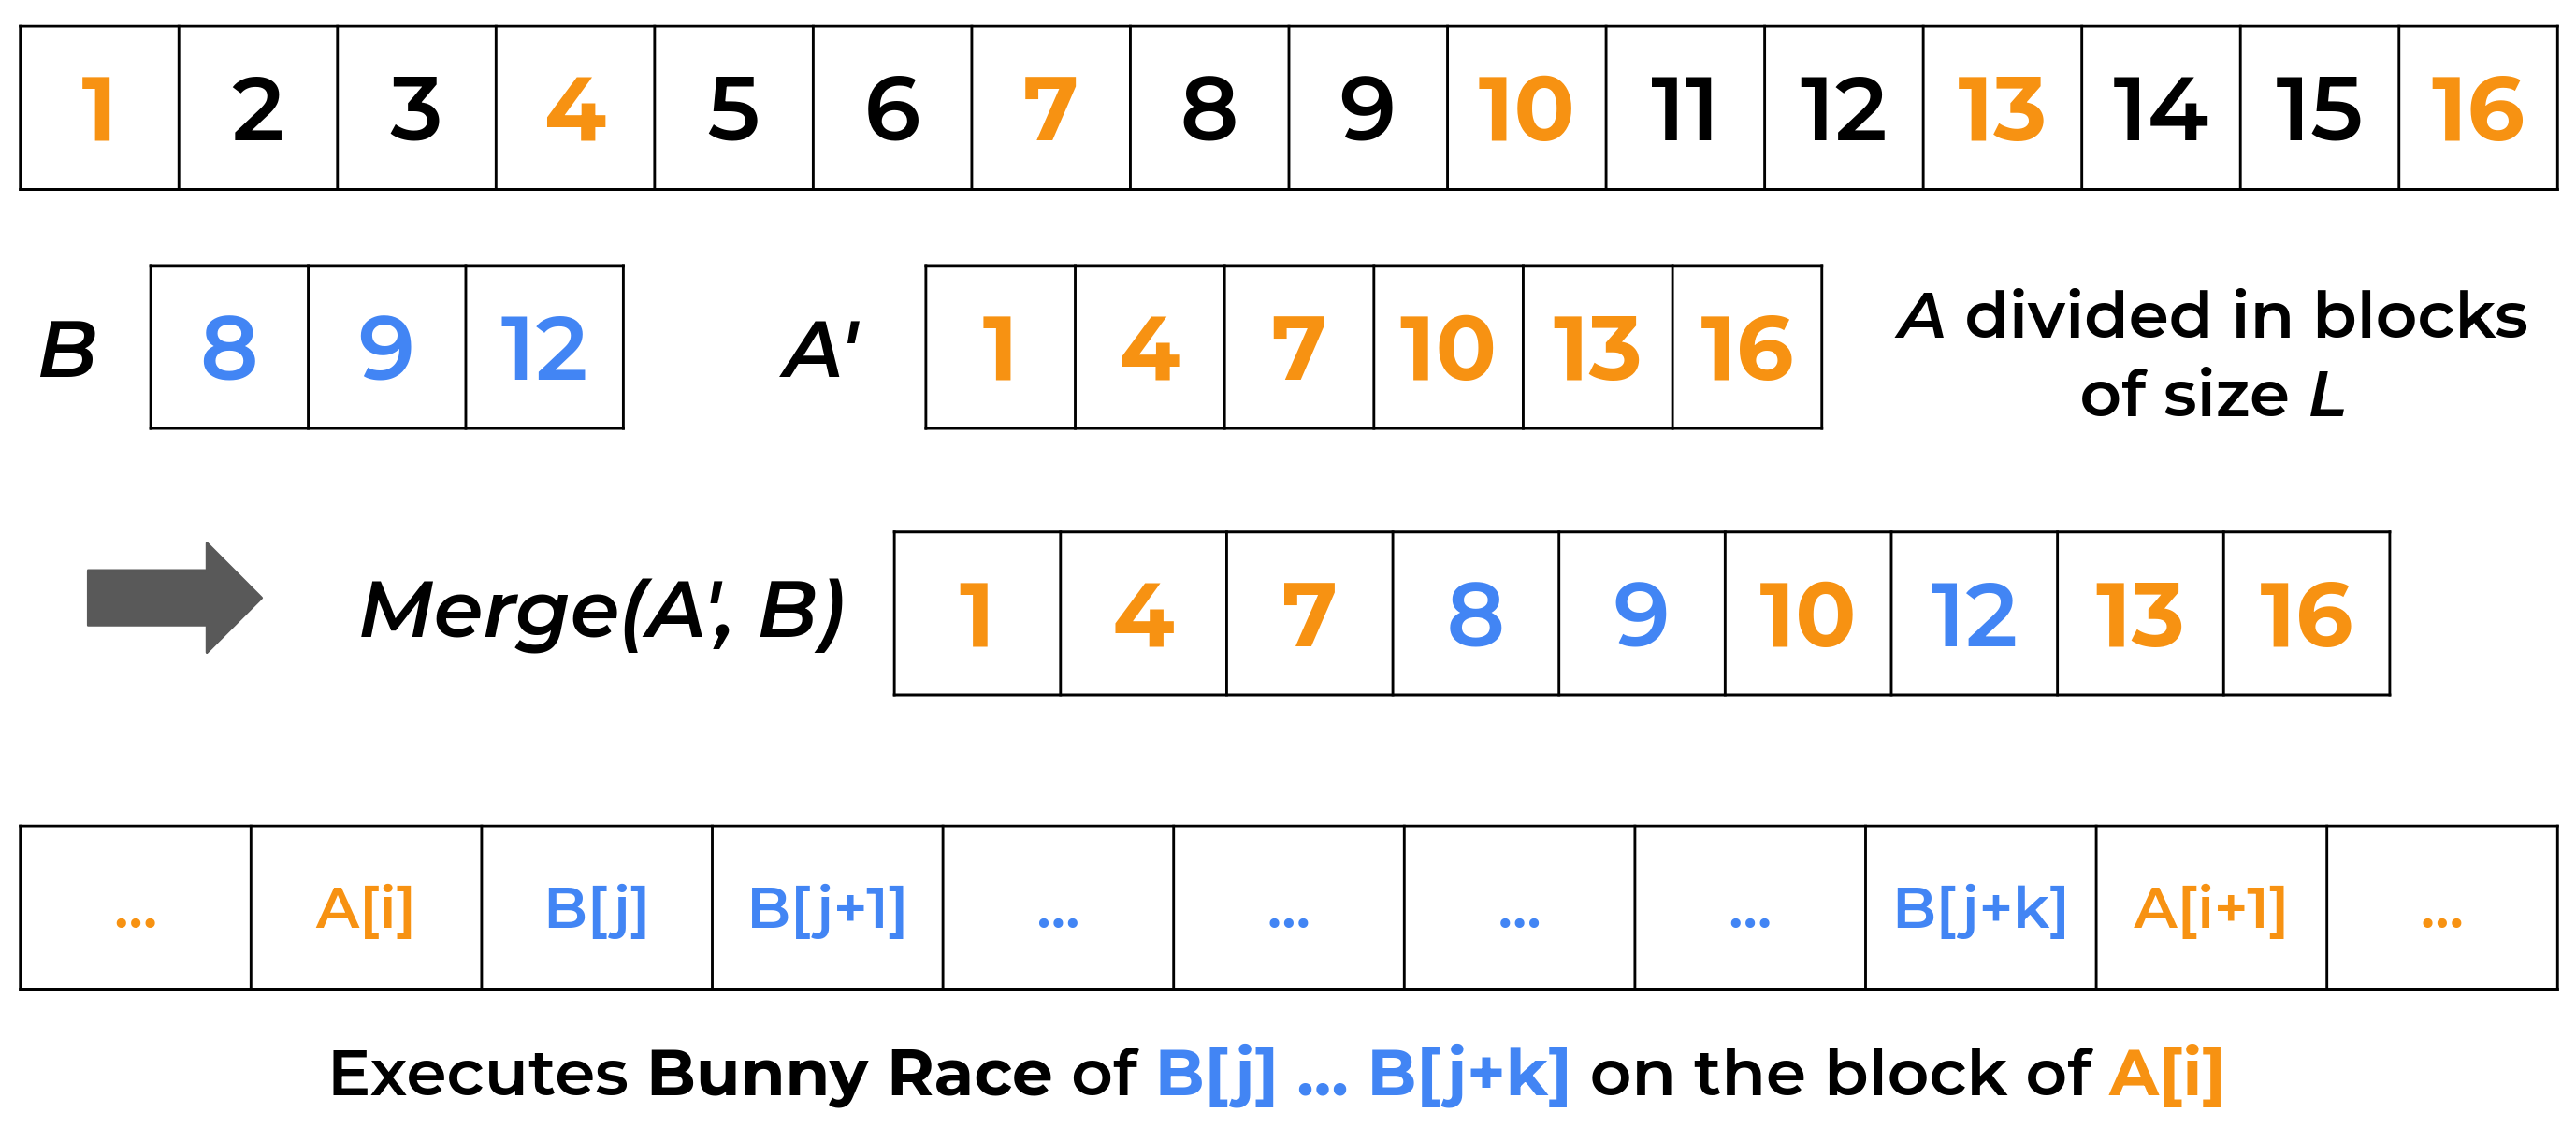
\includegraphics[width=.8\textwidth]{imgs/twolevel_storage.png}
        \caption{Two-level storage search algorithm \label{fig:twolevelstorage}}
    \end{center}
\end{figure}

Since most of the time we can consider physical memory as divided in two, namely cache and RAM, engineers took advantage of this by adopting a two-level storage approach: the main idea is to preprocess a collection of lists, logically partitioning each of them into blocks of size \textit{L} (final block may be shorter), and copying the first element of each block into an auxiliary sequence. Then, merge them and compute the intersection: elements of block $merged\_list[i+1]$ will be contained (if present) in block $merged\_list[i]$.\\
Let's see a simplified implementation where we preprocess only the longer sequence: say we have two lists such that $m=|B| \leq n=|A|$, we then divide \textit{A} in $\left\lceil \frac{n}{L} \right\rceil$ blocks of size \textit{L} and we save the first element of each block, called \textit{guides}, in a new list $A'$, effectively compressing the original list. \\
We then use the \textit{merge procedure} (which can be seen \href{https://en.wikipedia.org/wiki/Merge_algorithm}{here}) to merge $A'$ and \textit{B} into a new list \textit{Merged}, which will contain each \textit{guide} of \textit{A} and all elements of \textit{B} interspersed between them. The list is, of course, sorted.\\
Now we can find the elements of \textit{B} in the respective preceding \textit{guide} of \textit{A}. Lets clarify, we have:

\begin{itemize}
    \item $Merged[k] = A'[i]$
    \item $Merged[k+1 \ldots k+1+\alpha] = B[j \ldots j+\alpha]$
    \item $Merged[k+\alpha +2] = A'[i+1]$
\end{itemize}

Thus the elements of \textit{B}, $b_j \ldots b_{j+\alpha}$ can all be found in the block of \textit{guide} $A'[i]$.

Regarding time complexity, creating the list of \textit{guides} takes linear time over the size of \textit{A}. We then apply the \textit{merge procedure} to fuse together $A'$ and \textit{B} in $O\left(\frac{n}{L} +m \right)$ time, and finally we search for $b_j \ldots b_{j+\alpha}$ in the block of \textit{guide} $A[i]$ using the \textit{bunny race} \brref{sec:bunnyrace} algorithm in time $O\left(|A_i| + |B_j|\right) = O\left(L+|B_j|\right)$ where $|A_i|$ is the size of the block of $A'[i]$, and $|B_j| = \big|B[j \ldots j+\alpha]\big|$.\\
This algorithm is executed over all non-empty pairs $(A_i, B_j)$, which are no more than \textit{m} since $B = \cup_j B_j$, thus the total time taken by this step is $O(Lm+m)$.\\
Summing up the time complexity of all steps we get that the algorithm has:

\begin{itemize}
    \item $O \left( \frac{n}{L} +mL \right)$ Time complexity
    \item $O \left( \frac{n}{LB} + \frac{mL}{B} +m \right)$ I/Os 
\end{itemize}

Were \textit{B} is the disk-page size of the two-level memory model.

\section{Melding Algorithms}

"The algorithms discussed so far focus on intersecting two lists, even though they are easily extendable to \textit{k} lists intersections. Now we will see a collection of algorithms that can be used to intersect \textit{k} sets. Most of the algorithm shown are taken from the article "An Experimental Investigation of Set Intersection Algorithms for Text Searching" by Birbay and López-Ortiz \citep{birbay_ortiz}.

\subsection{Baeza-Yates and Baeza-Yates Sorted \label{sec:baezayates}}

One of the oldest algorithms presented in this survey, it is commonly found in the literature as a baseline for comparison, although it does not find much use in the real-world anymore. It was originally intended for the intersection of two sorted lists: it takes the median element of the smaller list and searches for it in the larger list, and it adds it to the result if it finds it.\\   
Since it will always find either and element (e.g. $b_j$) or a position where it could have been (e.g. $a_i \leq b_j \leq a_{i+1}$), it recursively calls itself on the two sub-lists in which each list can be split according to the median element. This approach is very similar to the \textit{divide and search} \brref{sec:divandsearch} algorithm.\\
To adapt this algorithm for \textit{k} sets, Baeza-Yates suggests to intersect the lists two-by-two, starting with the first two smallest ones. Since the result of the intersection may not be sorted, the result set needs to be sorted before going to the next list. The pseudocode can be seen at \textit{Algorithm} \brref{alg:baezayates}.

To avoid the cost of sorting each intermediate result, a minor variant can be used, called \textit{Baeza-Yates Sorted}, which move the elements to te result only at the last recursive step, ensuring they are added in order.

\begin{algorithm}
    \captionsetup{labelsep=newline}
    \caption{Pseudocode for Baeza-Yates algorithm \label{alg:baezayates}}
    \begin{algorithmic}[1]
        \Function{Baeza-Yates}{set,k}
            \State Sort sets by size \big($\big|set[0]\big| \leq \ldots \leq \big|set[k]\big|$\big)
            \ForAll{$i=1$ to $k$}
                \State $set[0] = BYinteresct\big(set[0], set[i], 0, \big|set[0]\big|-1, 0, \big|set[i]\big|-1\big)$
                \State Sort $set[0]$ 
            \EndFor
        \EndFunction

        \Statex

        \Function{BYintersect}{setA, setB, minA, maxA, minB, maxB}
            \If{$setA = \emptyset$ or $setB=\emptyset$}
                \State\Return $\emptyset$
            \EndIf
            \State Let $m=\frac{(minA+maxA)}{2}$
            \State Let $median\_A=setA[m]$
            \State Search for $median_A$ in $setB$
            \If{$median\_A$ found}
                \State Add $median\_A$ to result
            \EndIf
            \State Let $r$ be the position of $median\_A$ in $setB$
            \State Solve the intersection recursively on both sides of $r$ and $m$ in each set
        \EndFunction
    \end{algorithmic}
\end{algorithm}

\subsection{Sequential and Random Sequential \label{sec:sequential}}

\begin{wrapfigure}{r}{0.5\textwidth} %this figure will be at the right
    \centering
    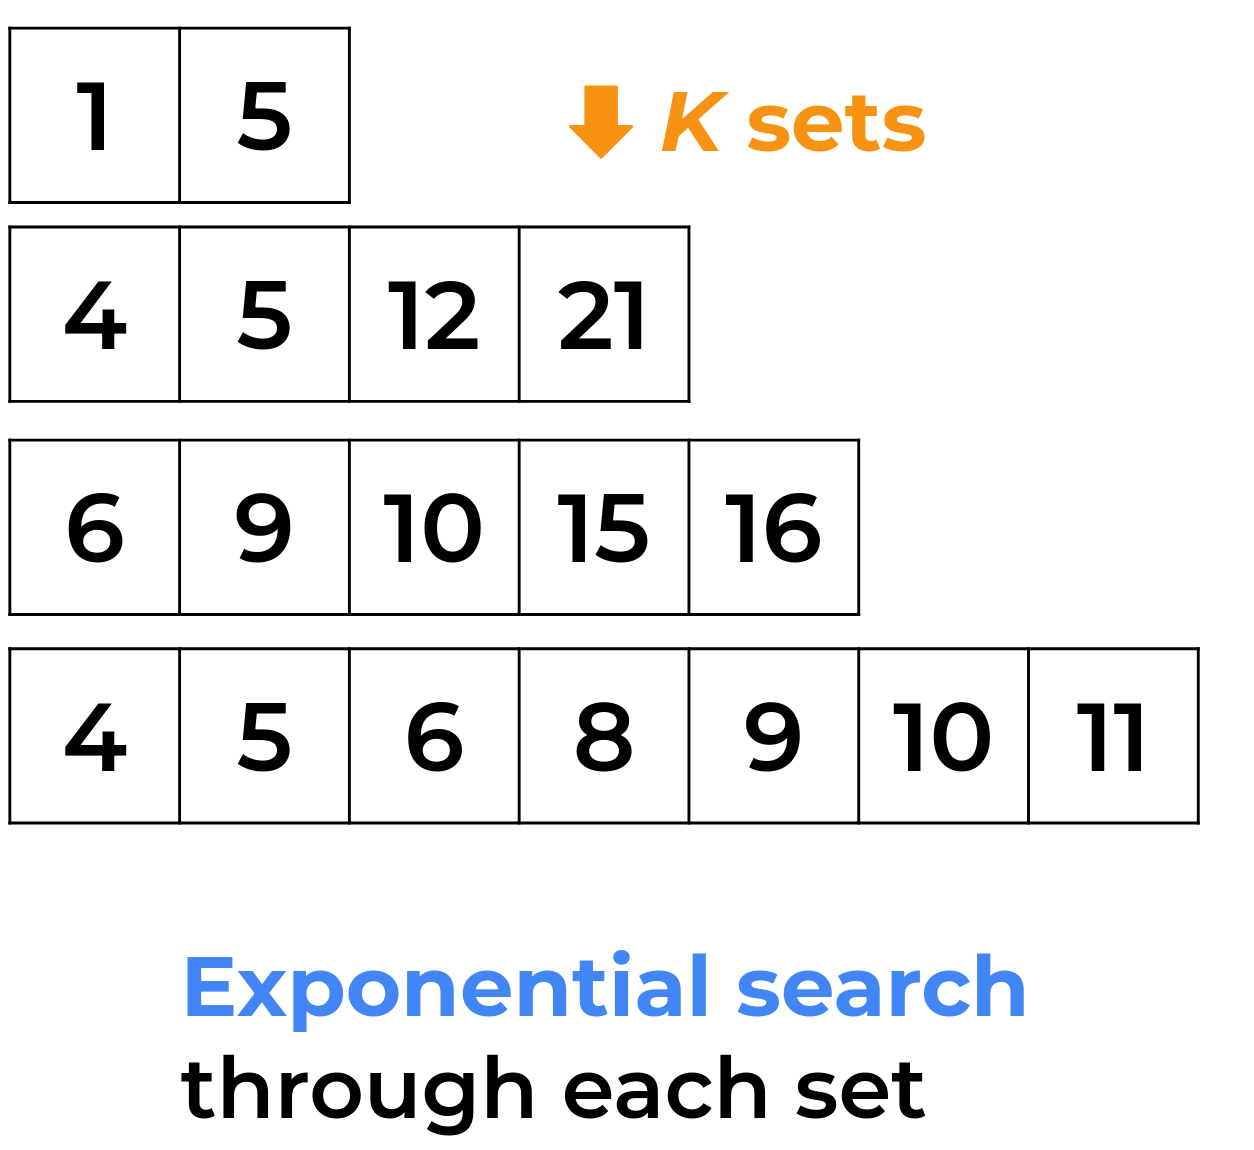
\includegraphics[width=.4\textwidth]{imgs/sequential.png}
    \caption{Sequential melding algorithm\label{fig:sequential}}
\end{wrapfigure}

Introduced by Barbay and Kenyon, it takes a collections of \textit{k} sorted sets ordered by size (ascending). Then it picks elements from the smallest one ($S_0$) and searches for them in the other sets ($S_{1 \ldots k-1}$) via \textit{galloping search} \brref{galloping}, one set at a time. It progressively check whether the element can be found in the set its looking into: if $key=1$ and $S_i[j]=7$ there is no need to keep checking $S_i$.
There exists a randomized variants which instead of going through the sets in order, it does so randomly (of course, it only chooses not-yet-checked sets).

The pseudocode of a simplified version can be seen at \textit{Algorithm} \brref{alg:sequential}, which has a time complexity of $O\left(k \cdot m^2 \left(1+ \log \frac{n}{m}\right)\right)$ since it performs \textit{k-galloping searches} for each element of the smallest set. We can let \textit{n} to be the size of the biggest list.\\
Another version of the algorithm, which considers also the eliminator and therefore is more efficient, can be seen at \textit{Algorithm} \brref{alg:sequential2}.

\begin{algorithm}
    \captionsetup{labelsep=newline}
    \caption{Pseudocode for Sequential melding algorithm \label{alg:sequential}}
    \begin{algorithmic}[1]
        \ForAll{$i=0$ to $|S_0|$}
            \State Let $key=S_0[i]$
            \State Let $counter=0$
            \ForAll{$j=1$ to $k-1$}
                \State \textit{Galloping search} for $key$ in $S_j$
                \If{$key$ found}
                    \State $counter = counter+1$
                \EndIf
            \EndFor
            \If{$counter=k-1$}
                \State Add $key$ to result
            \EndIf
        \EndFor
    \end{algorithmic}
\end{algorithm}

\begin{algorithm}
    \captionsetup{labelsep=newline}
    \caption{Pseudocode for Sequential with eliminator algorithm \label{alg:sequential2}}
    \begin{algorithmic}[1]
        \State Let eliminator be $e=S_0[0]$ 
        \State Let $i=1$
        \State Let $counter=0$
        \While{$e \neq \infty$}
            \State Search for $e$ in $S_i$
            \If{$e$ found}
                \State $counter=counter+1$
                \If{$counter=k-1$}
                    \State Add $e$ to result
                \EndIf
            \Else
                \State $e=S_i\left[succ(e)\right]$
            \EndIf
            \State $i=i+1$ mod $k$
        \EndWhile
    \end{algorithmic}
\end{algorithm}

\subsection{SvS and Swapping SvS \label{sec:svs}}

\begin{figure}[H] 
    \begin{center}
        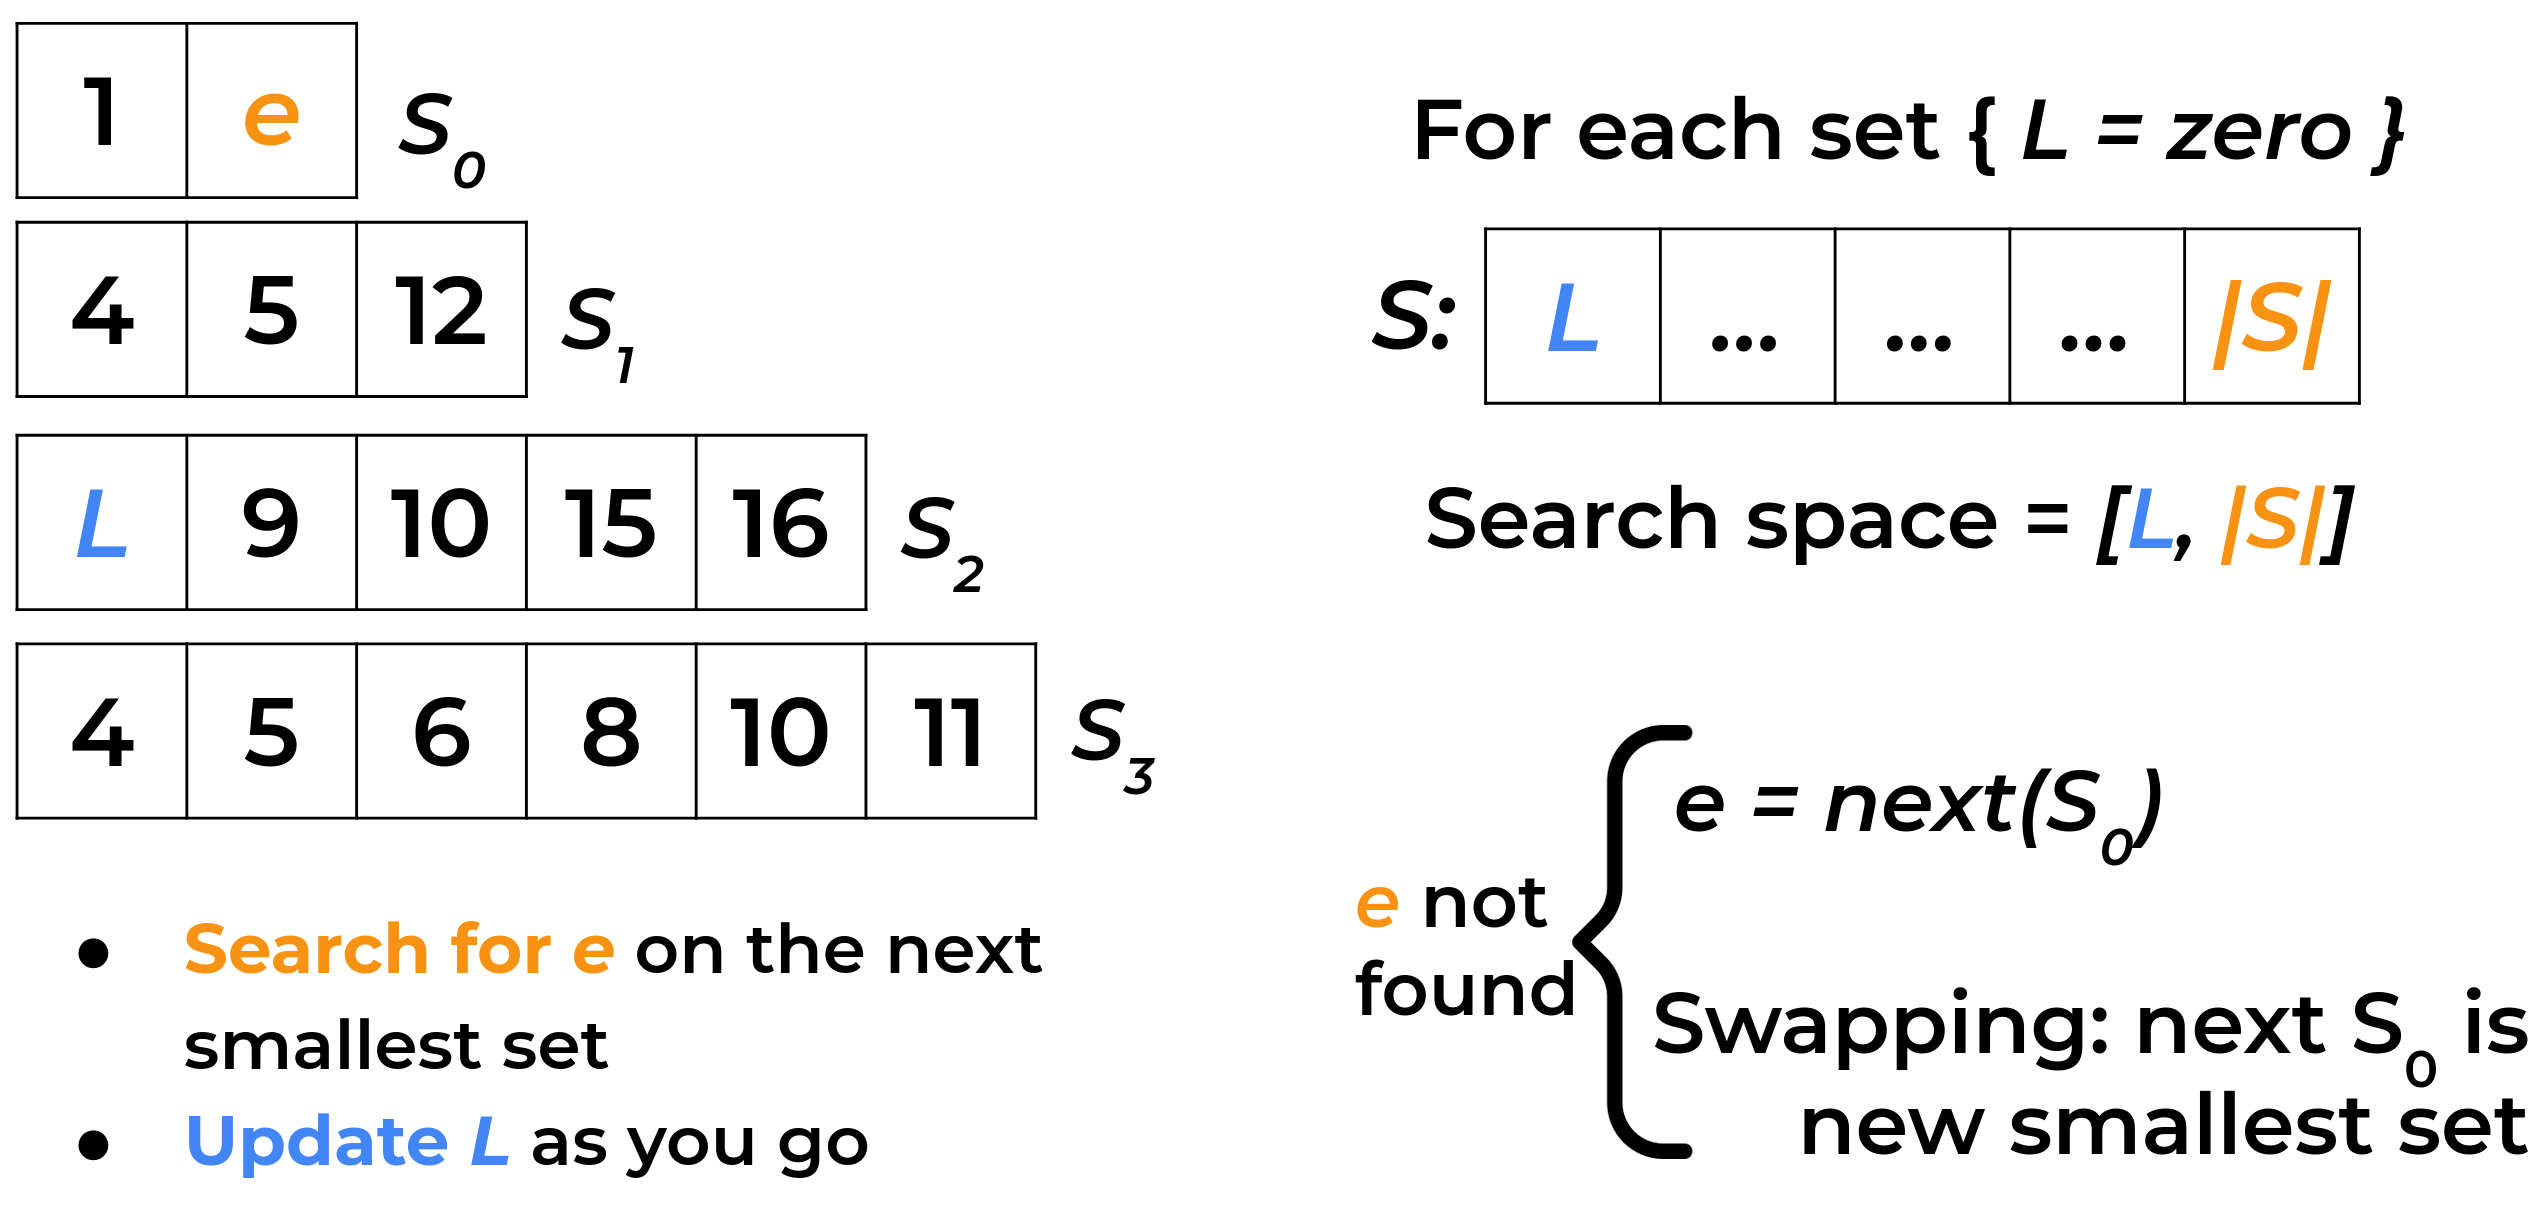
\includegraphics[width=.8\textwidth]{imgs/svs.png}
        \caption{SvS melding algorithm \label{fig:svs}}
    \end{center}
\end{figure}

\textit{SvS} is a widely used algorithm which, starting from a collection of sorted sets $S_0 \ldots S_k$, ordered by size (ascending), computes the intersection by iteratively reducing the search space.\\
We first instantiate a value $\ell=0$ for all sets, which will be used to keep track of the last checked element in each set, acting as a sort of logical starting position, then, we pick elements from the smallest set $S_0$ and search for them in the other sets, updating $\ell$ as we go: if $key=10$ and $S_j[\alpha]=9$ then we won't need to ever check $S_j[0 \ldots \alpha]$. We can use any search algorithm we want. \\
Its variant picks the next search element from the new smallest set instead than going through all the elements of the first smallest set (the "original" $S_0$).

The pseudocode of the algorithm can be seen at \textit{Algorithm} \brref{alg:svs}, and there is one thing worth noting: at the end of its run, the resulting intersection is contained in the smallest \textit{candidate} set $S_0$, wether such intersection exists (thus $S_0=[s_1, \ldots, s_\alpha]$) or not (thus $S_0= \emptyset$).

Once again, complexity is $O\left(k \cdot m^2 \left(1+ \log \frac{n}{m}\right)\right)$ if we decide to use the \textit{galloping search} \brref{galloping}, where $m=|S_0|$ and $n=|S_k|$, but since we update $\ell$ as we go, thus progressively reducing the search space, the algorithm is more efficient than \textit{Sequential} \brref{sec:sequential} in a real-world implementation.

\begin{algorithm}
    \captionsetup{labelsep=newline}
    \caption{Pseudocode for SvS melding algorithm \label{alg:svs}}
    \begin{algorithmic}[1]
        \State Sort sets by size \big($\big|set[0]\big| \leq \ldots \leq \big|set[k]\big|$\big)
        \ForAll{$i=0$ to $k-1$}
            \State Let $\ell[i]=0$ \Comment Set all starting positions to zero
        \EndFor
        \ForAll{$key$ in $S_0$}
            \ForAll{$i=1$ to $k-1$}
                \State Search for $key$ in $S_i$ in the range $\ell[i]$ to $|S_i|$
                \State Update $\ell[i]$ to the position of $key$ in $S_i$
                \If{$key$ not found}
                    \State Delete $key$ from $S_0$ \Comment $S_0$ is the result in the end
                \EndIf
            \EndFor
        \EndFor
    \end{algorithmic}
\end{algorithm}

\subsection{Small Adaptive \label{sec:smalladaptive}}

\begin{figure}[H] 
    \begin{center}
        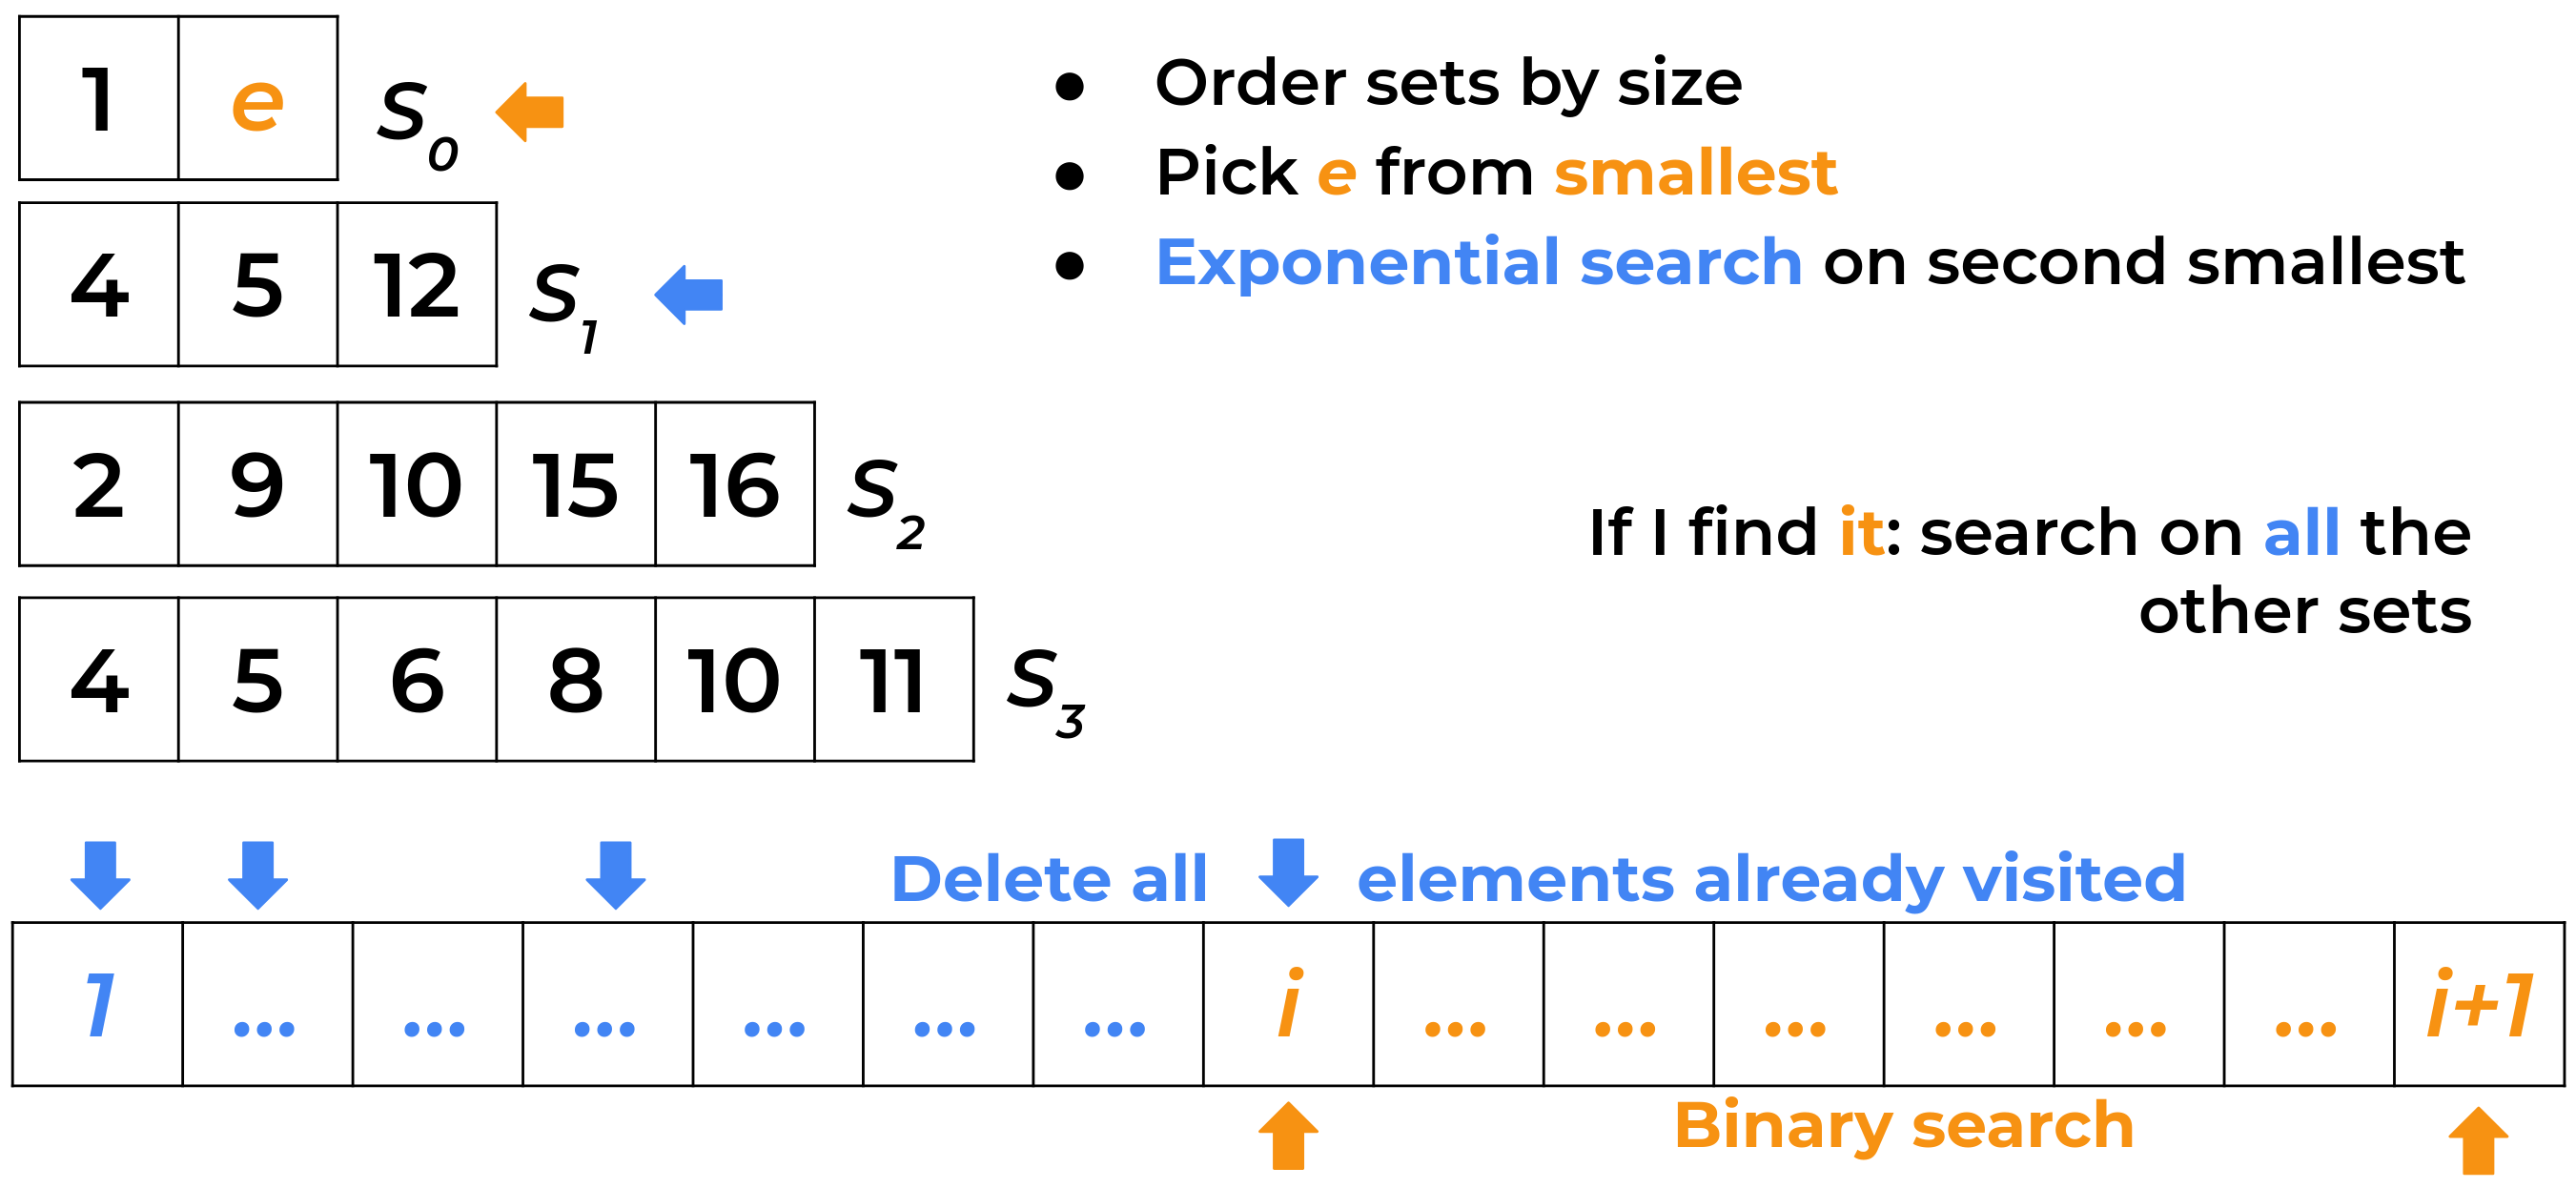
\includegraphics[width=.8\textwidth]{imgs/smalladaptive.png}
        \caption{Small Adaptive melding algorithm \label{fig:smalladaptive}}
    \end{center}
\end{figure}

Proposed by Birbay et al. in their article \citep{birbay_ortiz}, \textit{Small Adaptive} is a hybrid algorithm which combines properties from various others: we start from a collection of sets ordered by size (ascending), then we pick an element to search for (say $e$) from the smallest set $S_0$ and we perform an \textit{exponential search} \brref{sec:expsearch} on the second smallest set $S_1$. If we find it, we look for it in the remaining $k-2$ sets, deleting already-seen elements as we go, thus progressively reducing the search space. \\
The algorithm, after each search on a set $S_i$, picks the next smallest one and keeps ordering the sets so that, after a full search, it may be that $S_0$ and $S_1$ are different sets from before.

Pseudocode can be seen at \textit{Algorithm} \brref{alg:smalladaptive}, while the time complexity is almost identical to \textit{SvS} \brref{sec:svs} or \textit{Sequential} \brref{sec:sequential} (except for the ordering), but thanks to the ideas of: \textit{i.} searching first on the second smallest list before looking trough the rest; \textit{ii.} re-ordering the sets so we always first search into the two smallest and; \textit{iii.} deleting already-seen elements; \textit{Small Adaptive} can be more efficient in practice (although \textit{SvS} still outperforms it often). 

A comparison of the algorithms seen in \brref{sec:baezayates}, \brref{sec:sequential}, \brref{sec:svs} and \textit{Small Adaptive}, implemented and run on a collection of both synthetic and real-world-data datasets, can be seen in the tables: \ref{fig:birbay1}, \ref{fig:birbay2}, \ref{fig:birbay3}.

\begin{algorithm}
    \captionsetup{labelsep=newline}
    \caption{Pseudocode for Small Adaptive melding algorithm \label{alg:smalladaptive}}
    \begin{algorithmic}[1]
        \While{No set is empty}
            \State Sort sets by size \big($\big|set[0]\big| \leq \ldots \leq \big|set[k]\big|$\big)
            \State Look for $key=S_0[0]$
            \State Delete $S_0[0]$
            \State Let $couter=1$ \Comment At least $e \in S_0$ 
            \State Search for $key$ in $S_1$
            \If{$key$ found}
                \State $counter=counter+1$
                \ForAll{$i=1$ to $k-1$}
                    \State Search for $e$ in $S_i$
                    \State Delete already-seen elements 
                    \If{$key$ found}
                        \State $counter=counter+1$
                    \EndIf
                \EndFor
            \EndIf
            \If{$counter=k$}
                \State Add $key$ to result
            \EndIf
        \EndWhile
    \end{algorithmic}
\end{algorithm}

\begin{figure}[h] 
    \begin{center}
        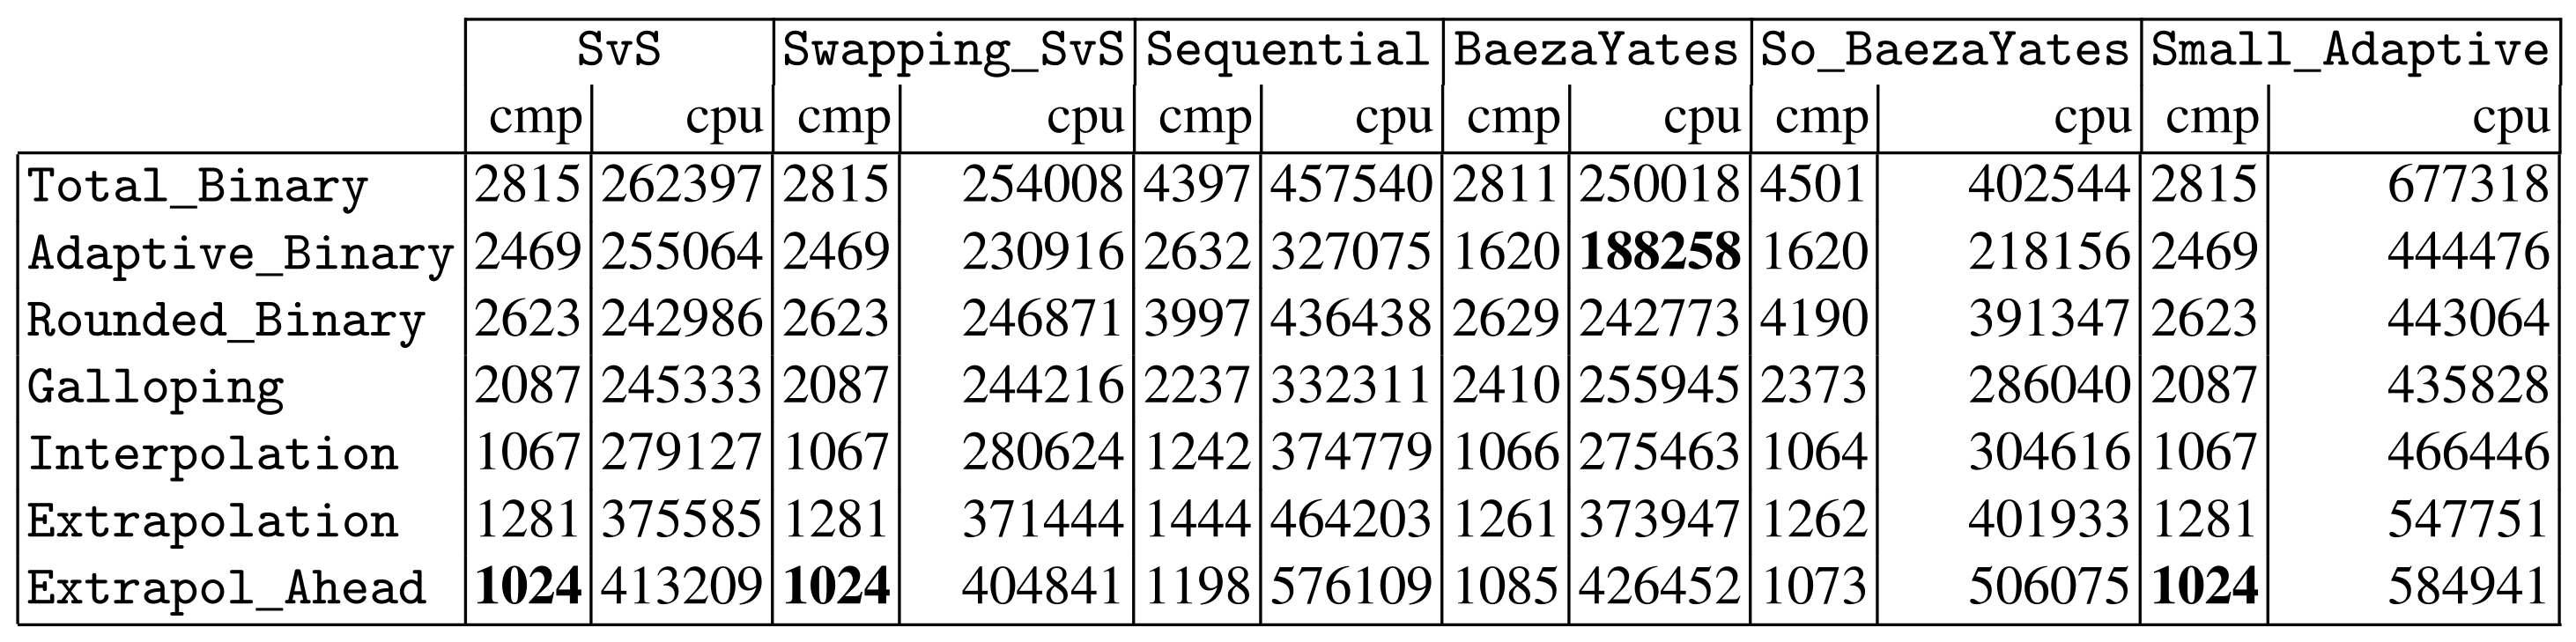
\includegraphics[width=.8\textwidth]{imgs/birbay_table3.png}
        \caption{Total number of comparisons and CPU times performed by each algorithm over the Random data set. In bold, the best
        performance in terms of the number of comparisons, for various melding algorithms in combination with \textit{Extrapol\_Ahead}, and
        the best performance in terms of CPU: \textit{BaezaYates} using \textit{Adaptive\_Binary}. \citep{birbay_ortiz} \label{fig:birbay1}}
    \end{center}
\end{figure}

\begin{figure}[h] 
    \begin{center}
        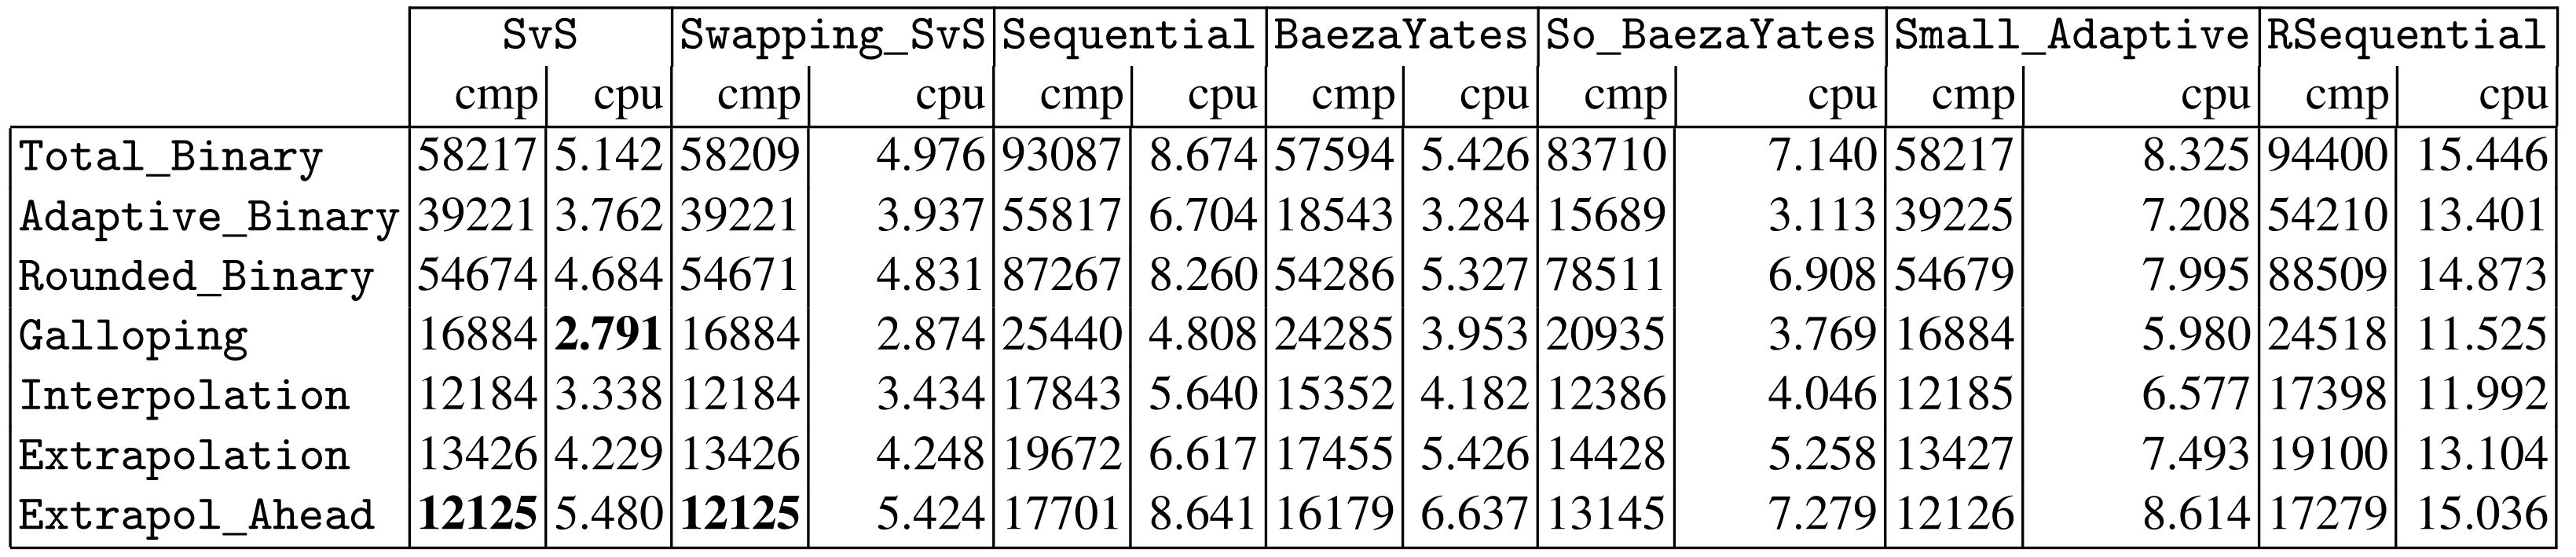
\includegraphics[width=.8\textwidth]{imgs/birbay_table5.png}
        \caption{Total number of comparisons and CPU times (in millions of cycles) performed by each algorithm over the Google data set.
        In bold, the best performance in terms of number of comparisons, \textit{SvS} and \textit{Swapping\_SvS} using \textit{Extrapol\_Ahead}, and in terms
        of CPU times, \textit{SvS} using \textit{Galloping}. \citep{birbay_ortiz} \label{fig:birbay2}}
    \end{center}
\end{figure}

\begin{figure}[h] 
    \begin{center}
        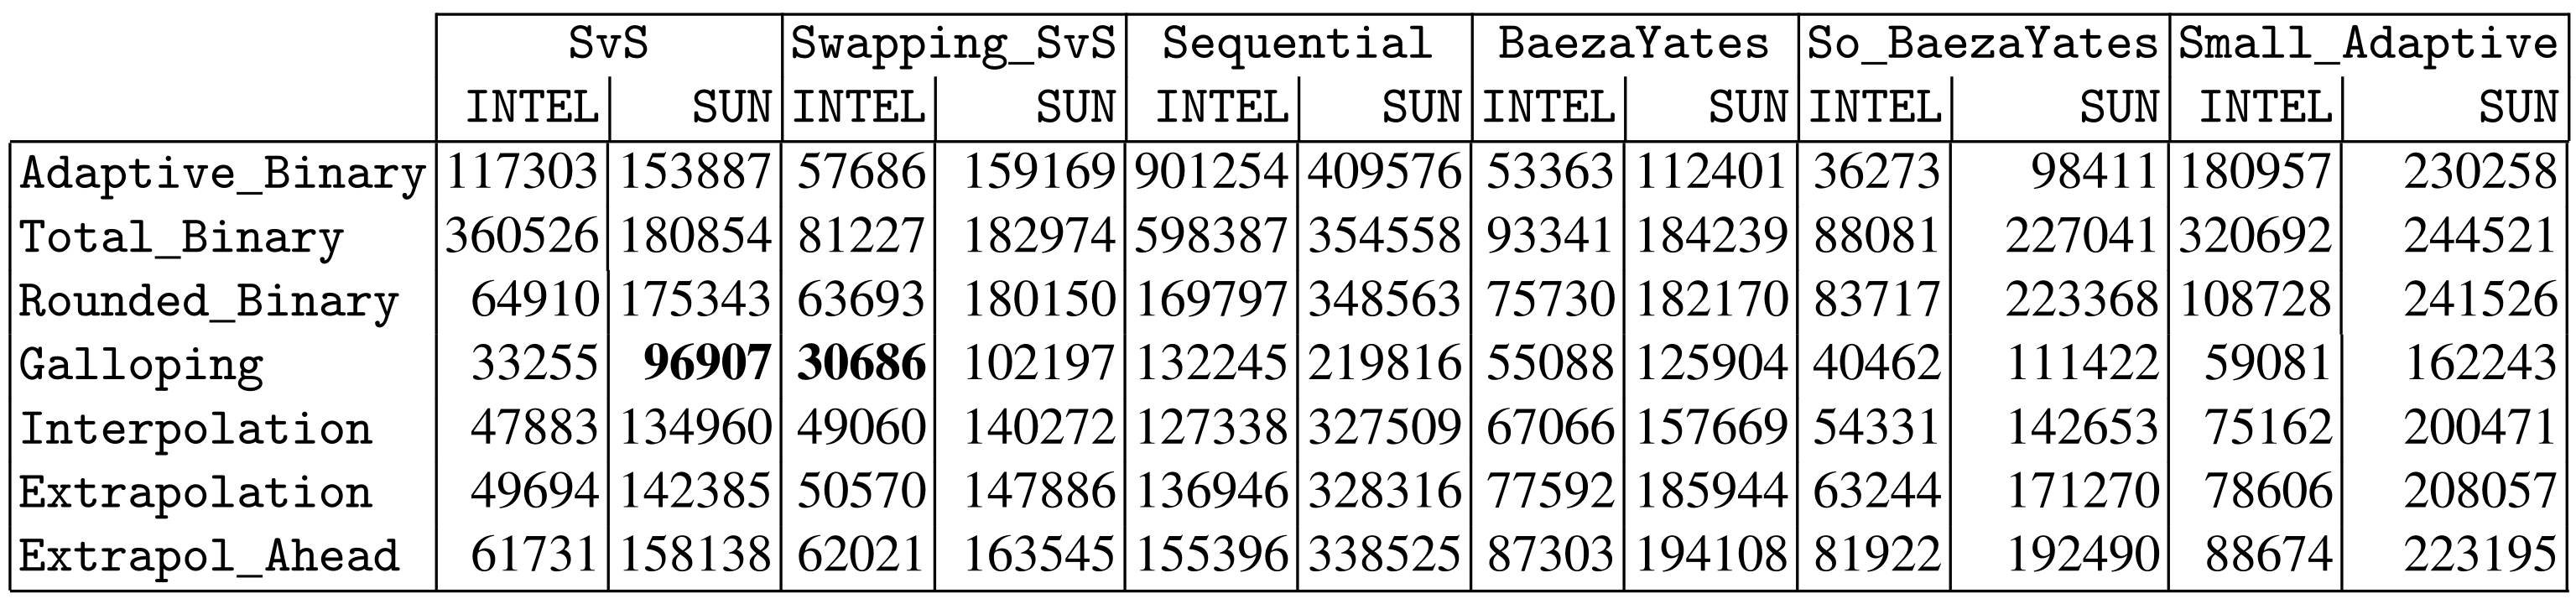
\includegraphics[width=.8\textwidth]{imgs/birbay_table7.png}
        \caption{Total CPU time performed by each algorithm over the TREC GOV2 data set. In bold, the smallest CPU times on the INTEL
        platform, obtained using \textit{Swapping\_SvS}; and on the SUN platform, obtained using \textit{SvS}, both in combination with \textit{Galloping}
        search. \citep{birbay_ortiz} \label{fig:birbay3}}
    \end{center}
\end{figure}